\chapter{Improved classification of microbiological aetiology in sepsis}
\label{ch:Results2}
\textit{This chapter explores the diagnosis of microbiological aetiology using various methods}

\startcontents[chapters]{\vspace{-1.4cm}}
\singlespacing
\printcontents[chapters]{}{1}{\section*{ }\setcounter{tocdepth}{1}}
\doublespacing

\section{Introduction}
\subsection{Clinical microbiology of the GAinS CAP cohort}
Of the 1222 patients with sepsis due to CAP in the GAinS cohort, a majority of 729 patients (60\%), were recorded as having no positive microbiology diagnosis (Table ~\ref{tab:clinmicro}). This figure compares similarly to that of the Etiology of Pneumonia in the Community (EPIC) study \parencite{Jain2015} which evaluated CAP requiring hospitalisation among adult patients in the USA and identified 62\% as lacking a microbiology diagnosis. 

\FloatBarrier
\begin{table}[]
\begin{center}
\begin{tabular}{|c|c|l|}
\hline
\multirow{2}{*}{\textbf{Diagnosis}} & \multicolumn{2}{c|}{\textbf{Number of patients (\%)}} \\ \cline{2-3} 
                                    & \textbf{GAinS (n=1222)}    & \textbf{EPIC (n=2259)}   \\ \hline
Unknown                             & 729 (60)                   & 1406 (62)                \\ \hline
Bacterial                           & 399 (33)                   & 247 (11)                 \\ \hline
Viral                               & 80 (7)                     & 530 (23)                 \\ \hline
Mixed bacterial/viral               & 12 (1)                     & 59 (3)                   \\ \hline
Fungal                              & 2 (0.2)                    & 17 (1)                   \\ \hline
\end{tabular}
\end{center}
\smallskip
\caption[GAinS Clinical microbiology classification] {\textbf{Microbiological classification for the GAinS (n=1222) and EPIC (n=2259) cohorts.} GAinS data based on curated electronic Case Record Form data. EPIC data obtained from the Etiology of Pneumonia in the Community Study \parencite{Jain2015}.} 
\label{tab:clinmicro}
\end{table}

Interestingly, the GAinS and EPIC cohorts differed in that bacterial infections were predominant in the GAinS cohort (33\%) whereas viral infections were predominant in the EPIC cohort (23\%). The most likely reason for the high viral diagnosis rate in the EPIC cohort is that all patients were systematically tested for viral infections by PCR on nasopharyngeal swabs whereas the GAinS cohort were tested according to clinician judgement. In addition, the higher prevalence of bacterial infections in the GAinS cohort may have been due to a higher severity of illness; GAinS recruited sepsis patients whilst EPIC recruited hospitalised CAP patients.

\subsection{GAinS electronic Case Record Form data}
The CAP microbiology section of the GAinS electronic Case Record Form (eCRF) is divided into three main sections (Figure \ref{fig:eCRF}). In this web-based form, research nurses are presented with a series of tick boxes and free text sections relating to:
\begin{enumerate}
	\item The name or category of any identified micro-organism.
	\item The source (sample type) of any identified micro-organism.
	\item Miscellaneous data (e.g. complicating factors such as presence of a pleural effusion, and vaccination status for pneumococcus/influenza).
\end{enumerate}

The eCRF aims to be simple in its format, unfortunately however, it lacks sufficient resolution to enable detailed microbiological phenotyping. For example, the eCRF format doesn't allow for a negative test result to be recorded, this is particularly relevant in the case of molecular testing for viral infections which are frequently not tested for. In addition, the eCRF does not allow for an identified organism to be matched to the source of the positive microbiological test, this is problematic if more than one organism is identified. Furthermore, one tick box option under source of positive microbiological test is "culture of lung secretions" which does not allow differentiation between an expectorated sputum sample and a directed broncho-alveolar lavage sample, samples with very different diagnostic values. The free text boxes of the eCRF often contained valuable clinical microbiology information. Thus, manual curation of the eCRF data was performed.

\subsection{Childhood Meningitis and Encephalitis Study (ChiMES) cohort} 
The targeted metagenomics work was performed in collaboration with the Childhood Meningitis and Encephalitis Study (ChiMES) investigators. ChiMES (http://www.encephuk.org/studies/ukchimes) is a UK-based multi-centre clinical study of over 3000 children with suspected meningitis and encephalitis. A subset of patients (n=243) were included in the targeted metagenomics aspect of the study, consisting of patients with a positive microbiological diagnosis (n=108) and patients without a microbiological diagnosis (n=135) (Table \ref{tab:chimesmicro}). A further control group of meningitis negative individuals (n=22, patients requiring a lumbar puncture for reasons other than meningitis) was studied.

\FloatBarrier
\begin{table}[]
\begin{center}
\begin{tabular}{|l|l|}
\hline
\textbf{Diagnosis}                & \textbf{Number of patients (\%)} \\ \hline
Unknown                           & 121 (50)                         \\ \hline
Enterovirus                       & 45 (19)                          \\ \hline
Human parechovirus                & 14 (6)                           \\ \hline
\textit{Streptococcus pneumoniae} & 15 (6)                           \\ \hline
\textit{Neisseria meningitidis}   & 13 (5)                           \\ \hline
Other                             & 35 (15)                          \\ \hline
\textbf{Total}                    & \textbf{243}                     \\ \hline
\end{tabular}
\end{center}
\smallskip
\caption[ChiMES clinical microbiology classification] {\textbf{Microbiological classification for the ChiMES (n=243) cohort.} These diagnoses were made from routine clinical microbiological testing of CSF and/or blood.} 
\label{tab:chimesmicro}
\end{table}

\subsection{Digital droplet PCR (ddPCR)}
Digital droplet PCR (ddPCR) is a method which utilises water-oil emulsion droplet technology. In this technique, a droplet generation step is performed which partitions a 20$\mu$l sample into approximately 20,000 nanolitre-sized droplets. The principle is that each droplet contains one or no copies of the target molecule and the PCR reaction occurs simultaneously in each droplet containing the target molecule. Advantages of ddPCR include absolute quantification without the need for a standard curve (Poisson statistics are employed), increased precision due to the degree of sample partitioning, and increased signal-to-noise ratio where the relative concentration of target to background is low. 

ddPCR was chosen as a method to be applied to the GAinS samples for several reasons. Firstly, it provided an independent method for evaluating the performance of \textit{Castanet}. This is particularly applicable because a clinical microbiological diagnosis of a particular infection type would not necessarily mean the organism was present in plasma, both because the original diagnosis could have arisen from a different specimen type and also because the plasma sampled for metagenomics was collected after antibiotic administration. Secondly, ddPCR provided a quantitative method of assessing pathogen load in plasma.

\subsection{Random forests}
Random forests \parencite{Breiman2001} are supervised machine learning algorithms which are capable of performing both regression and classification tasks. A forest is created which consists of a number of decision trees. Each decision tree sees a subset of the training data (bootstrapping) and at each decision node, a random sample of \textit{m} predictors is chosen from the full set of \textit{p} predictors. For classification tasks, each tree votes for a class and the forest chooses the class which has the most votes by the majority of trees in the forest. Advantages of random forests leading to their suitability for classification tasks based on (meta)genomic data include their ability to handle missing values, their robustness to overfitting, and their ability to handle large datasets with high dimensionality. 

\subsection{Axiom Microbiome Array}
The Axiom Microbiome Array (Affymetrix) is a commercially available platform that enables detection of all organisms in a sample. Organisms are identified at species- or strain-level resolution within a single reaction. The platform is based on microarray technology, with 1,277,846 target probes and 60,152 random negative control probes. The target probes represent 135,555 sequences from 12,513 microbial species from five domains: archaea, bacteria, fungi, protozoa and viruses. 

\subsection{Aims}

To improve microbiological classification of GAinS sepsis patients with CAP through:
\begin{enumerate}
	\item Application of targeted metagenomics to plasma samples
	\item Use of droplet digital PCR (ddPCR) to assay \textit{Streptococcus pneumoniae} and Epstein-Barr Virus from plasma samples
	\item Use of the Axiom Microbiome Array
\end{enumerate}

\section{Results}

\subsection{Targeted metagenomics}
\textbf{Large scale analysis of clinical samples.}
There was successful sequencing of a total of 854 individuals, derived from 243 ChiMES meningitis cases, 27 non-meningitis negative-control CSF samples, 573 GAinS sepsis cases, and 11 negative-control plasma samples (Figure ~\ref{fig:samples}). The 243 meningitis included 122 patients for which a pathogen had been identified by clinical microbiology (108 from CSF only, plus 14 from a blood sample +/- CSF) and 121 where no pathogen had been identified before sequencing. The sepsis cases comprised 126 for which a pathogen had been identified and 447 chosen for the study because no pathogen had been identified in any relevant sample. The clinical characteristics for the 573 GAinS CAP sepsis cases are summarised in Table ~\ref{tab:clin-gains}.

\FloatBarrier
\begin{figure}[htbp]
\centering
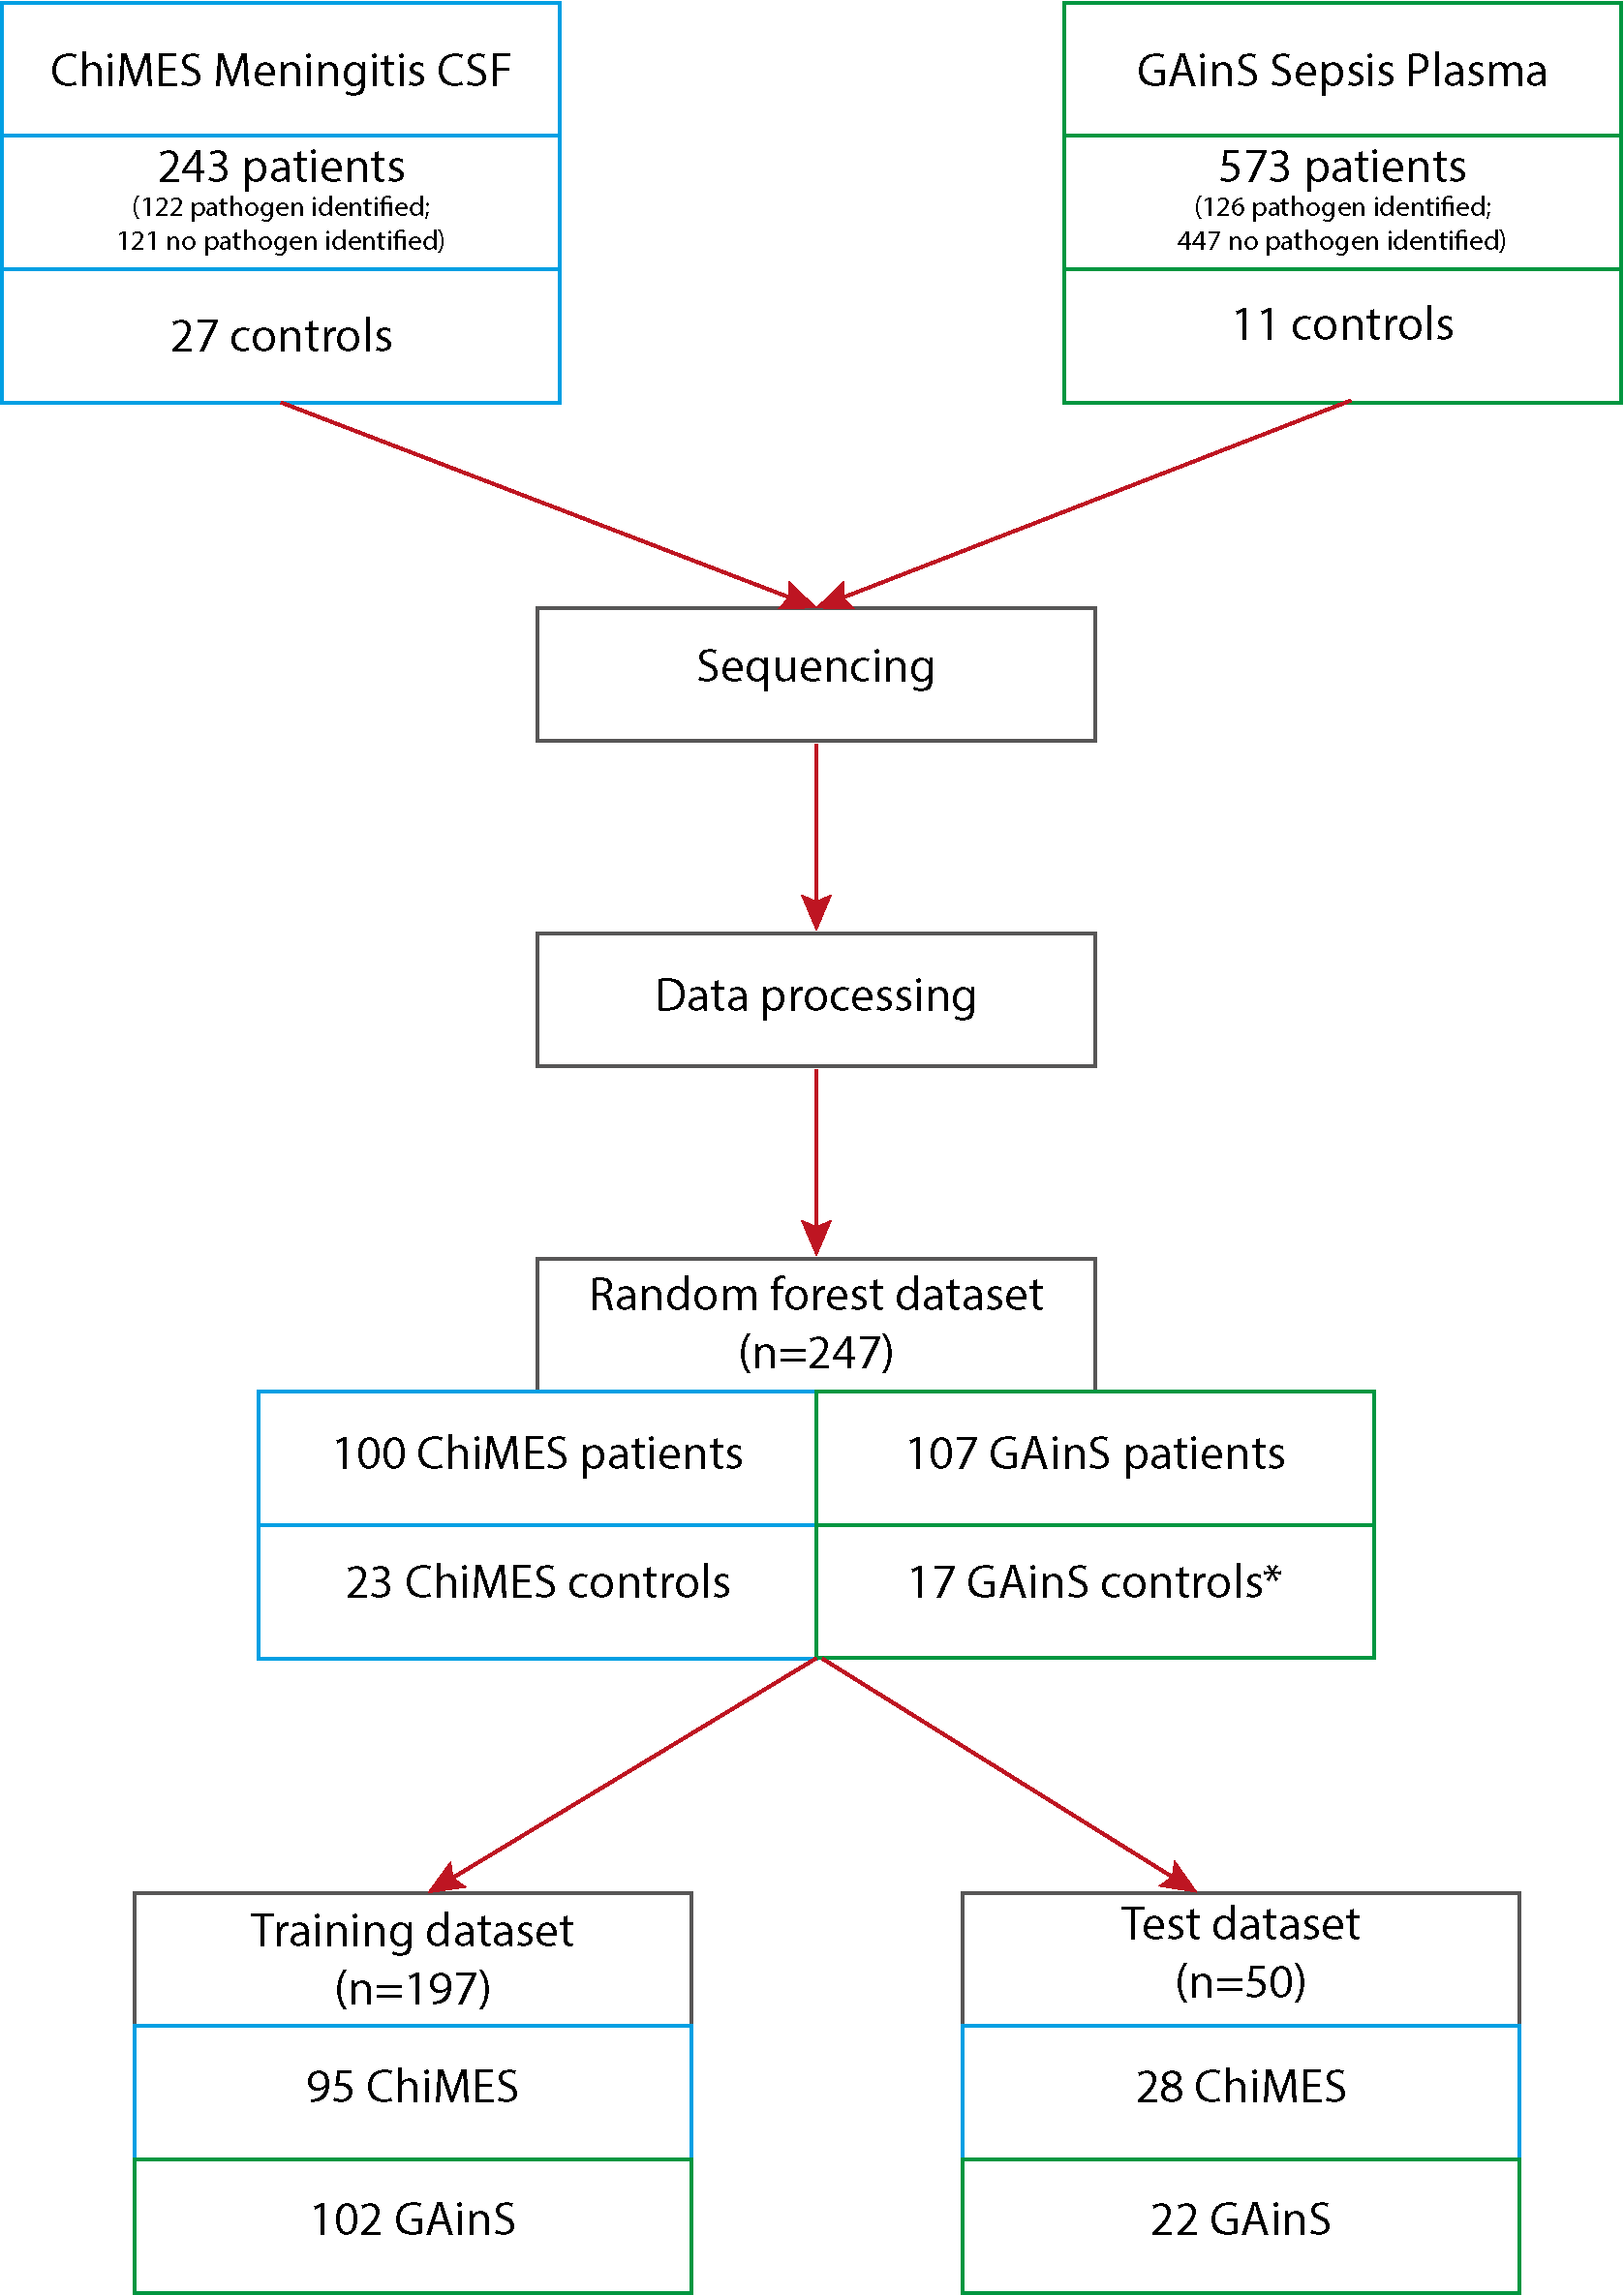
\includegraphics[scale=0.8]{./Results2/Images/flowchart.png}
\caption[Flowchart of samples analysed]{\textbf{Flowchart of samples analysed.} Samples undergoing targeted metagenomic sequencing are detailed in the flowchart. Control samples for ChiMES are CSF samples obtained from individuals without meningitis/encephalitis. Control samples from GAinS are plasma samples obtained from non-infected individuals undergoing elective cardiac surgery. CSF samples are outlined in blue and plasma samples are outlined in green. Samples used to train and test the random forest algorithm are detailed in the flowchart. *The number of GAinS control samples in the random forest dataset (17) exceeds the number of patients detailed initially (11) because several patient samples were split into several aliquots and sequenced.}
\label{fig:samples}
\end{figure}

\FloatBarrier
\begin{table}[]
\begin{center}
\begin{tabular}{|l|l|}
\hline
\textbf{Characteristic}      & \textbf{GAinS cohort (n=573)}                                                                     \\ \hline
Age (years)                  & 61                                                                                                \\ \hline
Male sex                     & 324 (57\%)                                                                                        \\ \hline
Charlson comorbidity index   & 1.1                                                                                               \\ \hline
Mortality (28-day)           & 121 (21\%)                                                                                        \\ \hline
ICU length of stay (days)    & 9.9                                                                                               \\ \hline
SOFA score (day 1)           & 6.2                                                                                               \\ \hline
SOFA score (maximum)         & 7.1                                                                                               \\ \hline
Mechanical ventilation       & 460 (80\%)                                                                                        \\ \hline
Vasopressors                 & 297 (52\%)                                                                                        \\ \hline
Earliest ICU day of sampling & \begin{tabular}[c]{@{}l@{}}Day 1: 302 (53\%); Day 3: 192 (34\%); \\ Day 5: 79 (14\%)\end{tabular} \\ \hline
\end{tabular}
\end{center}
\smallskip
\caption[Clinical characteristics of GAinS metagenomic cohort]{\textbf{Clinical characteristics of GAinS metagenomic cohort (n=573)} Mean or count data is summarised for the various clinical characteristics. ICU length of stay excludes patients who died in ICU. Earliest day of sampling refers to the earliest timepoint at which a plasma sample was collected for metagenomic analysis.}
\label{tab:clin-gains}
\end{table}

\textbf{Development of random forest algorithm.}
In order to evaluate the ability of \textit{Castanet} to identify pathogens in real clinical samples, a 'truth dataset' of samples was compiled whose status for particular pathogens was known with confidence. For meningitis cases, the pathogen identified by clinical microbiology testing was accepted as the truth state for microbiology-positive samples. For the 126 pathogen-positive CAP sepsis cases, the pathogen identification had often been made in a sample other than plasma and most of the plasma samples in the collection had been obtained after administration of antibiotics, two situations in which plasma levels of pathogens might have been undetectable by any method. Accordingly, a positive result by ddPCR for \textit{S. pneumoniae} or Epstein-Barr virus (EBV) was used to define a sample subset with which to learn the characteristics of pathogen-true-positive sequencing data. 

Another key issue in interpreting metagenomic sequencing data, especially in large pools of samples, is to distinguish low-level positives from true-negative samples. Here, the \textit{S. pneumoniae} ddPCR assays were used to estimate the threshold for considering a sample sequence-positive. Samples with fewer than either 72 total (specificity 0.94, sensitivity 0.83) or 4 de-duplicated (specificity 0.84, sensitivity 0.85) sequence reads from any single pathogen were excluded from consideration as sequencing-positive (i.e. they were not considered by the random forest algorithm) (Figure \ref{fig:strep-threshold}).

\FloatBarrier
\begin{figure}[htbp]
\centering
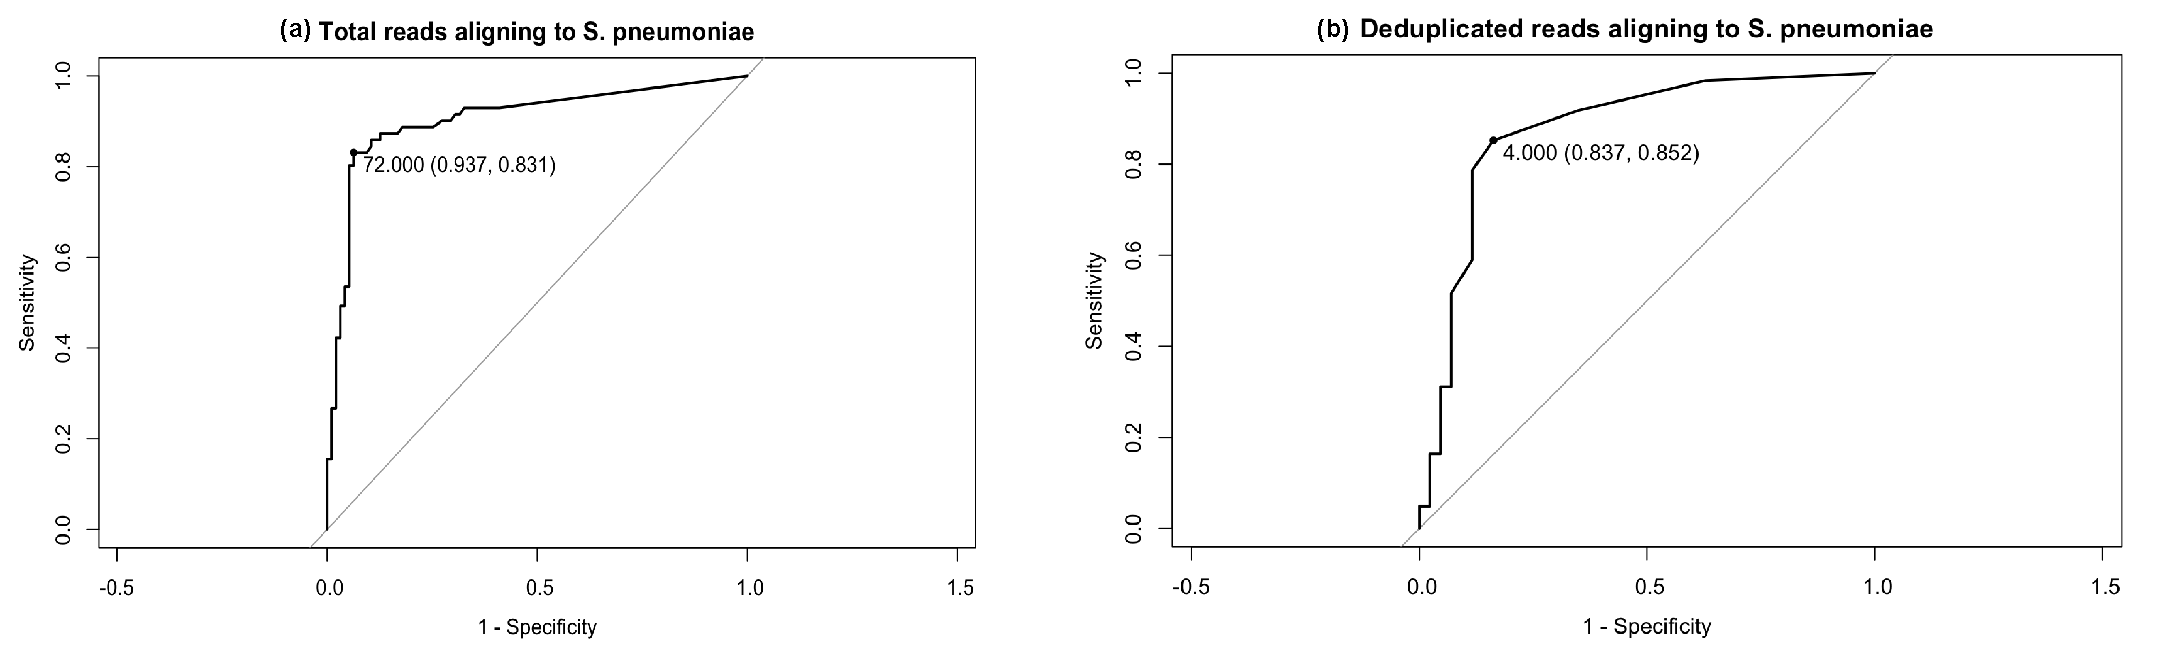
\includegraphics[scale=0.8]{./Results2/Images/strep-threshold.png}
\caption[\textit{S. pneumoniae} detection thresholds in GAinS samples]{\textbf{\textit{S. pneumoniae} detection thresholds in GAinS samples.} Sample read statistics were assessed as predictors of ddPCR-positive status for \textit{S. pneumoniae} detection. ROC curves of (a) total reads and (b) de-duplicated reads as predictors are presented here. Youden's J statistic was used to select the respective thresholds of 72 total reads (specificity 0.94, sensitivity 0.83) and 4 de-duplicated reads (specificity 0.84, sensitivity 0.85) for calling a sample positive.}
\label{fig:strep-threshold}
\end{figure}

Combining the above criteria, 100 ChiMES meningitis CSF and 107 GAinS sepsis plasma samples were identified for inclusion as samples with known pathogen status. In addition, negative control samples were included in this cohort (CSF from non-meningitis patients, n=23; plasma from sepsis-negative patients, n=17) to provide instances of pathogen-negative data. Plasma and CSF samples that were microbiology-positive for a particular pathogen were deemed negative for other pathogens. Reads aligning to viruses known to reactivate in sepsis (herpes simplex virus, cytomegalovirus, human herpes virus 6, JC virus) were excluded from the analysis, apart from those EBV samples where ddPCR data was available.

The 247 samples defined above were randomly allocated to training and test datasets in an 80:20 ratio. The training dataset (197 samples: 95 CSF; 102 plasma) were used to train a random forest classifier that used a set of variables derived from the sequencing data to derive a score between 0 and 1 to indicate whether it was positive for each organism with reads in a sample. Most samples contained reads from multiple organisms and the random forest returns a score for each one of these organisms.

The test dataset comprised 50 samples (28 CSF; 22 plasma). A cut-off random forest score of 0.465 was selected for classification of the test set, to appropriately weight specificity over sensitivity (Figure \ref{fig:rf-roc}). At this threshold, there were five false negatives and one false positive in the ChiMES test dataset and one false negative and three false positives in the GAinS test dataset. In the combined set of test samples (Figure ~\ref{fig:rf-test}), the sensitivity was 86.7\% (39 of 45 true positives) and the specificity was 98.6\% (283 of 287 true negatives). Among the most informative sequencing data metrics for prediction were the numbers of total and de-duplicated reads matching a pathogen, taken as the respective proportions of reads aligning to all pathogens in the probeset, and whether a high proportion of the targeted region (regions in the probeset) for that pathogen were covered by reads. 

Since excluding pathogens from a diagnosis can also be clinically useful, the performance of the method in predicting negative status was assessed. With a random forest score threshold of 0.015, 59.2\% of true negatives were correctly identified, with a specificity of 97.8\%, implying that for many samples it is possible to exclude many possible pathogens without erroneously ruling out true positives.

\FloatBarrier
\begin{figure}[htbp]
\centering
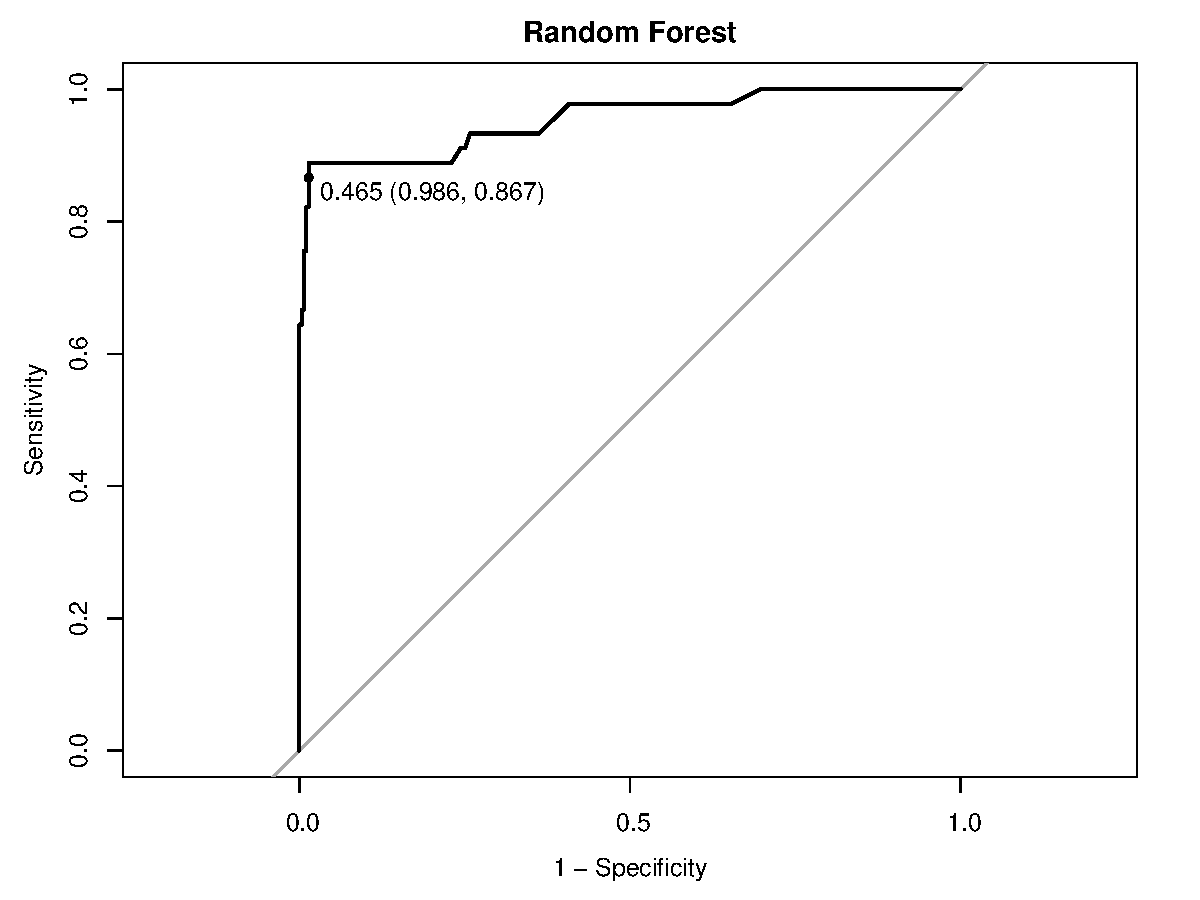
\includegraphics[scale=0.6]{./Results2/Images/rf-roc.pdf}
\caption[Random forest ROC curve]{\textbf{Random forest ROC curve.} ROC curve derived from random forest training dataset (n=197; ChiMES n=95, GAinS n=102) to choose random forest score threshold for predicting positive samples. A threshold of 0.465 was selected to call samples as positive for a particular pathogen. At this threshold, specificity was 0.986 and sensitivity 0.867.}
\label{fig:rf-roc}
\end{figure}

\begin{figure}[htbp]
\centering
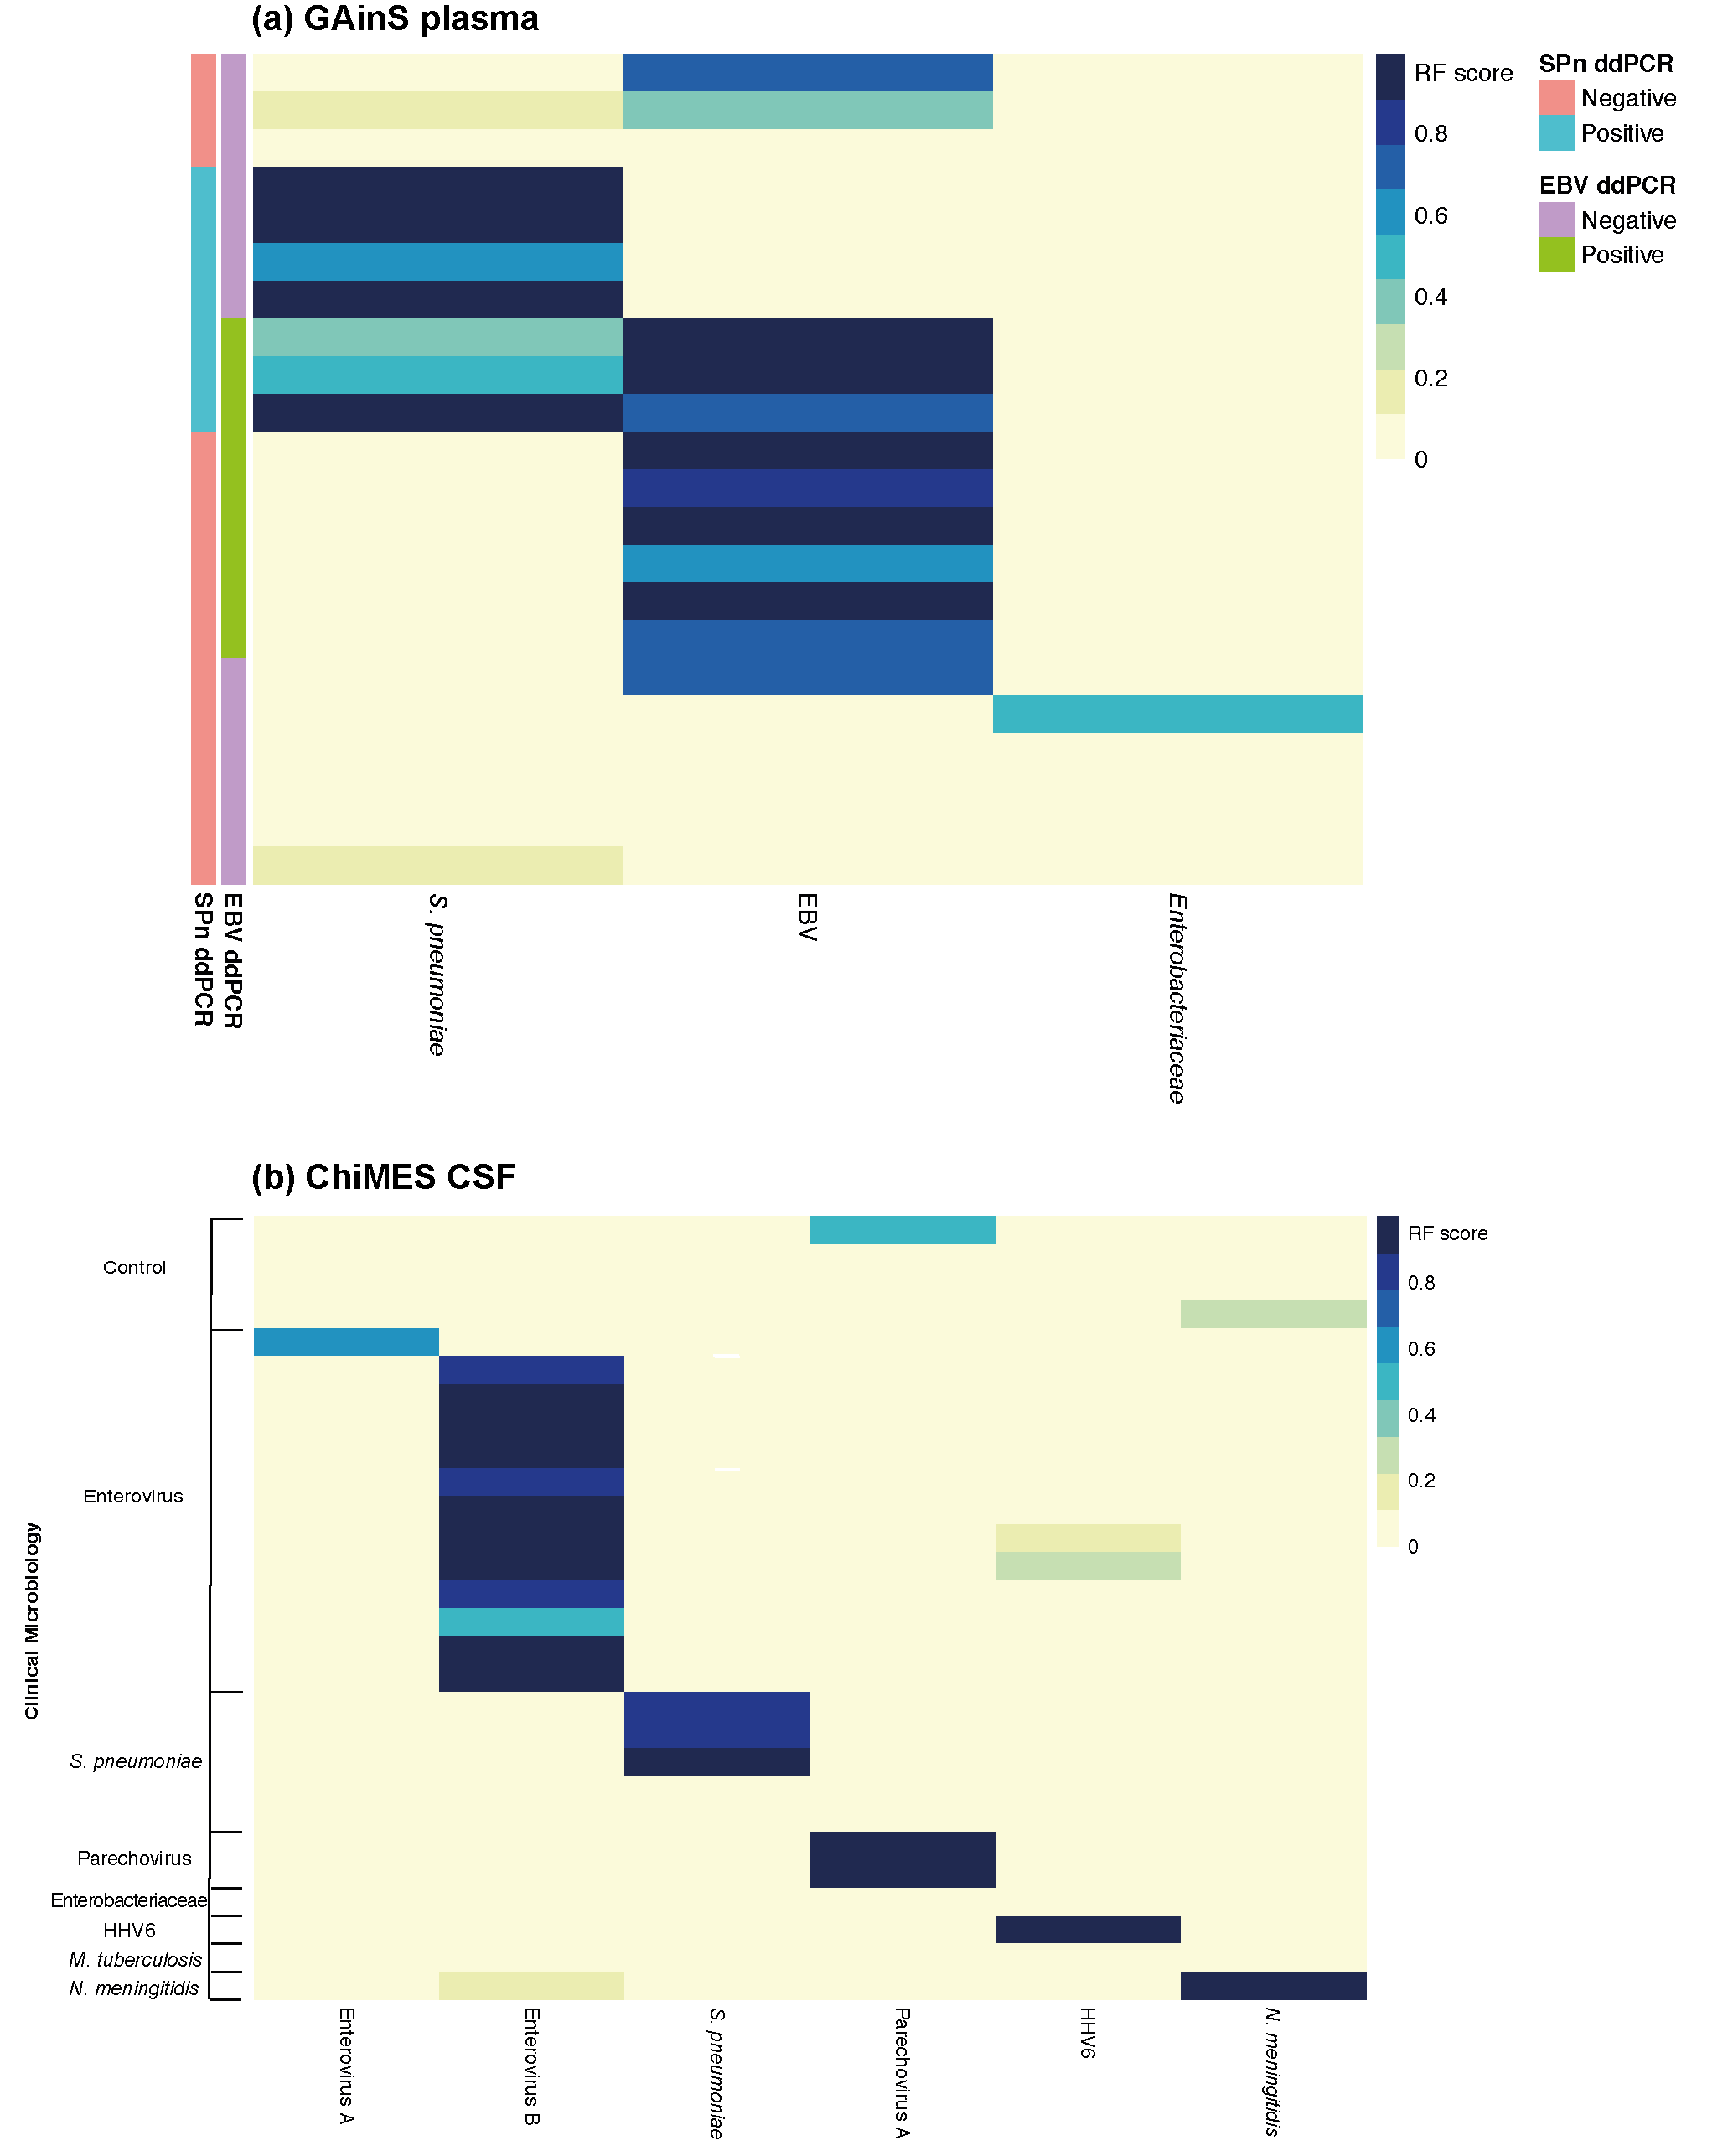
\includegraphics[scale=0.9]{./Results2/Images/rf-test.png}
\caption[GAinS/ChiMES test dataset]{\textbf{GAinS/ChiMES test dataset.} Performance of \textit{Castanet} in clinical samples with a positive microbiology diagnosis. The test dataset included 50 samples: (a) 22 plasma samples (20 GAinS, 2 sepsis-negative controls); (b) 28 CSF samples (24 ChiMES, 4 meningitis-negative controls). The combined overall test dataset specificity and sensitivity was 0.986 and 0.867 respectively. Only organisms detected in each sample set are included as columns in each panel. RF=random forest; HHV6=human herpes virus 6; SPn=\textit{Streptococcus pneumoniae}; EBV=Epstein-Barr Virus; TB=\textit{Mycobacterium tuberculosis}; ddPCR=droplet digital PCR.}
\label{fig:rf-test}
\end{figure}
\FloatBarrier

\textbf{Application to samples with no previous microbiology diagnosis.}
Of the 729 GAinS patients with sepsis due to CAP that had no known microbiological diagnosis (Table ~\ref{table:clinmicro}), 447 had plasma available for analysis. In this group of samples, in which no causative pathogen had been identified by routine clinical microbiology, \textit{Castanet} identified one or more pathogens in 37\% of samples (n=165), including both bacteria and viruses that in many cases were likely to have been causative (Figure ~\ref{fig:rf-unknown}). Among such pathogens, instances of EBV, human herpes virus 6, herpes simplex virus, JC virus and cytomegalovirus in sepsis may represent viral reactivation in the context of critical illness, while \textit{Burkholderia cerpacia} and \textit{Nocardia asteroides} sequences have been previously noted to represent contamination of samples \parencite{Salter2014}. Excluding these likely reactivations and contaminants, \textit{Castanet} made 50 new detections in sepsis patients, comprising 11\% of previously unresolved cases (Table ~\ref{tab:gains-unknown}). 

Correspondingly, in the ChiMES samples, \textit{Castanet} made 39 new detections (32\%) of clinically relevant pathogens in the 121 meningitis patients with negative clinical microbiology. 
 
\begin{figure}[htbp]
\centering
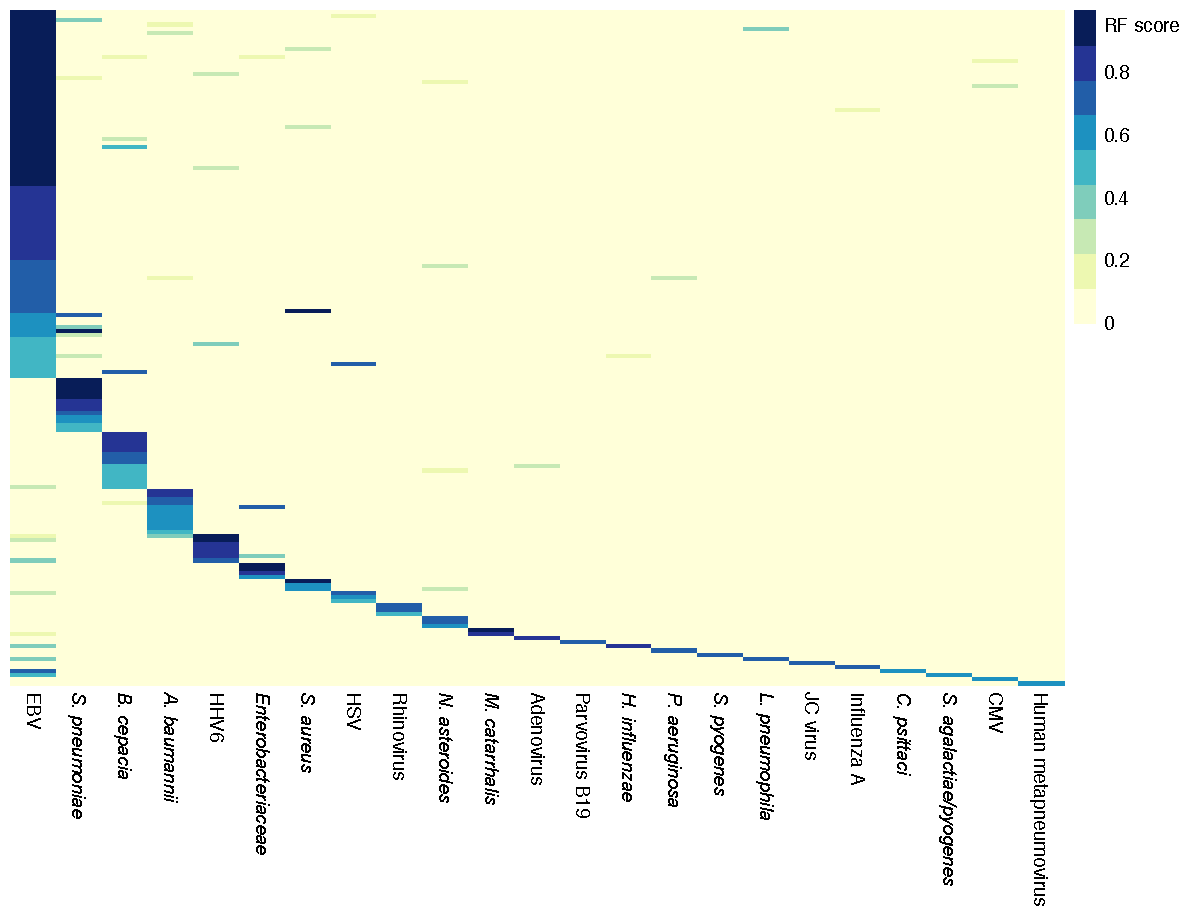
\includegraphics[scale=0.8]{./Results2/Images/rf-gains-unknown.pdf}
\caption[GAinS cases with no clinical microbiology diagnosis]{\textbf{Performance of \textit{Castanet} in GAinS CAP sepsis cases with no clinical microbiology diagnosis.} The heatmap depicts samples from patients with no microbiological diagnosis where at least one organism was detected at a random forest (RF) score $>$0.465 (n=165/447). Only organisms detected in each sample set are included as columns in the heatmap.}
\label{fig:rf-unknown}
\end{figure}
\FloatBarrier

\begin{table}[]
\begin{center}
\begin{tabular}{|c|c|}
\hline
\textbf{Organism}                 & \textbf{Number of patients} \\ \hline
\textit{Streptococcus pneumoniae} & 16                          \\ \hline
\textit{Acinetobacter baumannii}  & 11                          \\ \hline
\textit{Enterobacteriaceae}       & 5                           \\ \hline
\textit{Staphylococcus aureus}    & 4                           \\ \hline
\textit{Moraxella catarrhalis}    & 2                           \\ \hline
\textit{Haemophilus influenza}    & 1                           \\ \hline
\textit{Pseudomonas aeruginosa}   & 1                           \\ \hline
\textit{Streptococcus pyogenes}   & 1                           \\ \hline
\textit{Legionella pneumophila}   & 1                           \\ \hline
\textit{Chlamydia psittaci}       & 1                           \\ \hline
Rhinovirus                        & 3                           \\ \hline
Adenovirus                        & 1                           \\ \hline
Parvovirus B19                    & 1                           \\ \hline
Influenza A                       & 1                           \\ \hline
Human metapneumovirus             & 1                           \\ \hline
\textbf{Total}                    & \textbf{50}                 \\ \hline
\end{tabular}
\end{center}
\smallskip
\caption[New pathogens identified by \textit{Castanet}] {\textbf{New pathogen identifications made by \textit{Castanet} among sepsis plasma samples.} } 
\label{tab:gains-unknown}
\end{table}



\subsection{Digital droplet PCR in GAinS samples}
ddPCR was performed on GAinS samples with sepsis due to CAP as an independent method for evaluating the performance of \textit{Castanet} and also to enable quantitative evaluation of pathogen load in the samples.

\textbf{\textit{Streptococcus pneumoniae}.} ddPCR for the \textit{S. pneumoniae cpsA} gene (conserved in nearly all 90 known serotypes of \textit{S. pneumoniae} \parencite{Morona2004}) was performed on the following samples:
\begin{enumerate}
	\item 139 samples from 92 patients with \textit{S. pneumoniae} infection diagnosed by clinical microbiology.
	\item 15 samples from 15 patients with no microbiology diagnosis.
	\item 4 samples from 4 patients with influenza infection diagnosed by clinical microbiology.
\end{enumerate}

ddPCR was performed on the latter two groups of samples for cross-validation because \textit{S. pneumoniae} reads had been unexpectedly identified on metagenomic sequencing. This was prior to the development of the \textit{Castanet} random forest algorithm, thus the remainder of this section will focus only on the ddPCR result from the 92 patients with \textit{S. pneumoniae} infection diagnosed by clinical microbiology.

Of the 139 samples tested, 47 (33.8\%) were positive for \textit{S. pneumoniae}. ddPCR results were compared with \textit{Castanet} sequencing (Table \ref{tab:ddpcr-castanet}). If ddPCR is considered as the gold standard result, this would mean Castanet has a specificity of 100\% and a sensitivity of 83\% for \textit{S. pneumoniae}. There was no significant association between ddPCR positivity and blood culture positivity for \textit{S. pneumoniae} ($\chi^2$=0.13, d.f.=1, p=0.72).

\begin{table}[]
\begin{center}
\begin{tabular}{|l|l|l|l|l|}
\hline
\multicolumn{2}{|l|}{\multirow{2}{*}{}} & \multicolumn{2}{l|}{Castanet} & \multirow{2}{*}{Total} \\ \cline{3-4}
\multicolumn{2}{|l|}{}                  & Negative      & Positive      &                        \\ \hline
\multirow{2}{*}{ddPCR}    & Negative    & 92            & 0             & 92                     \\ \cline{2-5} 
                          & Positive    & 8             & 39            & 47                     \\ \hline
\multicolumn{2}{|l|}{Total}             & 100           & 39            & 139                    \\ \hline
\end{tabular}
\end{center}
\smallskip
\caption[ddPCR and Castanet results for \textit{S. pneumoniae}] {\textbf{ddPCR and Castanet results for \textit{S. pneumoniae in GAinS CAP sepsis samples}}. Comparison of results in samples with both ddPCR and \textit{Castanet} data (n=139 samples from n=92 patients).} 
\label{tab:ddpcr-castanet}
\end{table}

\textbf{Epstein-Barr virus.} ddPCR was performed on 619 samples from 565 patients for Epstein-Barr virus (EBV). See Section ~\ref{sssec:ebv}.

\textbf{Influenza virus.} ddPCR was performed for the influenza A matrix gene on 14 plasma samples from 14 patients. All patients had been diagnosed with influenza infection by PCR of a nasopharyngeal swab or respiratory specimen. All samples were negative for influenza via \textit{Castanet} and also tested ddPCR negative. 

\textbf{Relationship between organism load and sequencing yield} Similar to the finding for the five quantified VMR viruses (Figure \ref{fig:vmrconc}), a linear relationship between input pathogen load and sequencing yield was observed in a subset of sepsis plasma samples for which bacterial and viral load of \textit{S. pneumoniae} (n=102) and EBV (n=199) respectively had been quantified by ddPCR (Figure \ref{fig:ddPCR}). Samples where both the ddPCR result and sequencing reads were zero were excluded from the analysis. These findings indicate that the number of de-duplicated reads obtained from targeted enrichment provides data on quantitative yield.

\FloatBarrier
\begin{figure}[htbp]
\centering
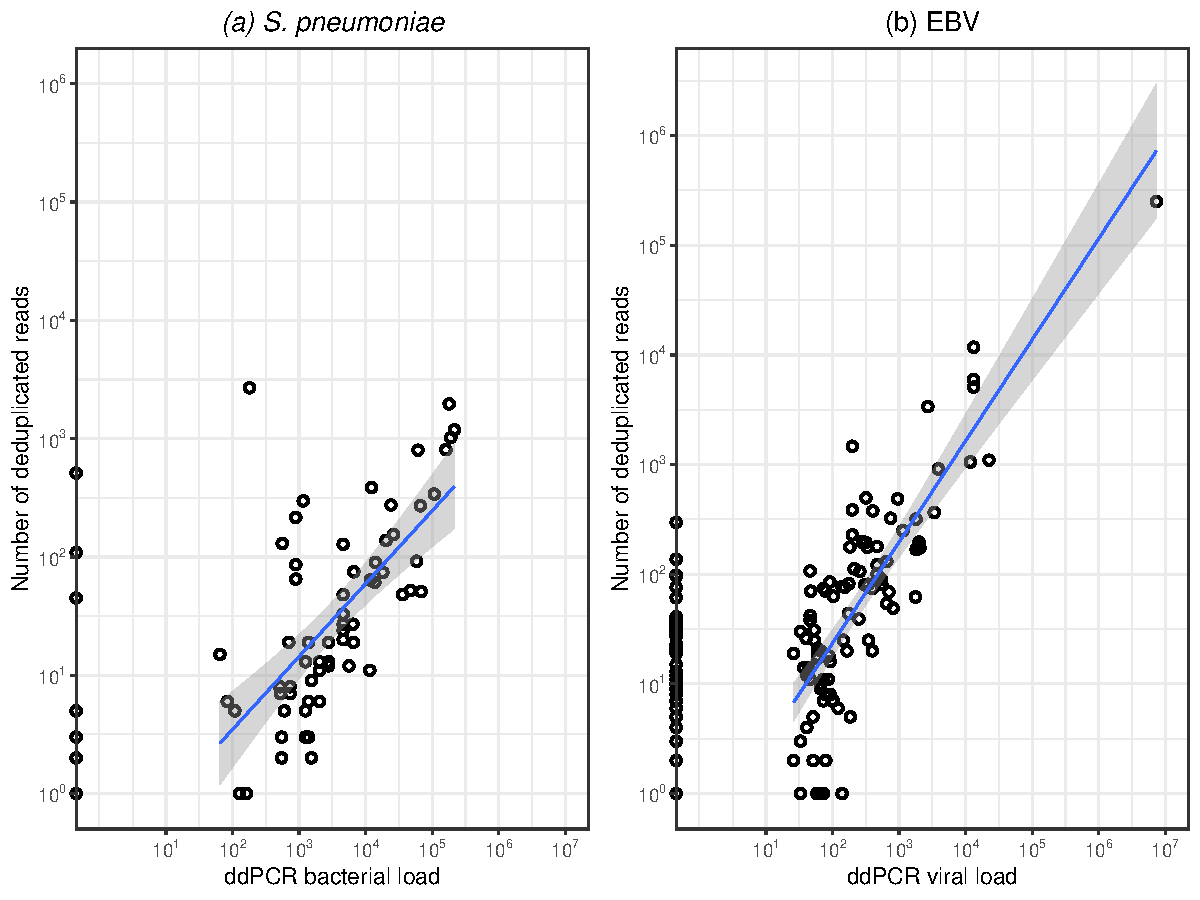
\includegraphics[scale=0.6]{./Results2/Images/ddPCR.pdf}
\caption[Organism load and sequencing yield in sepsis samples]{\textbf{Organism load and sequencing yield in sepsis samples.} De-duplicated read yield was plotted against pathogen load, estimated by ddPCR in samples from a subset of cases in which (a) \textit{Streptococcus pneumoniae} (n=102) or (b) Epstein-Barr virus (EBV) (n=199) was detected by sequencing. A linear relationship between pathogen load and sequencing yield was observed for each organism (\textit{S. pneumoniae}: Pearson's R$^2$ = 0.449, p = 8.8 x 10$^{-5}$; EBV: Pearson's R$^2$ = 0.702, p = 2.9 x 10$^{-16}$.)}
\label{fig:ddPCR}
\end{figure}

\subsection{Axiom Microbiome Array}
We evaluated plasma from ten patients on the Axiom Microbiome Array platform (Affymetrix). This included four patients with \textit{S. pneumoniae} CAP sepsis, three patients with influenza CAP sepsis, and three uninfected cardiac surgery controls. The Axiom Microbiome Array was evaluated only in terms of detection for DNA-based pathogens as limited sample availability meant that RNA in the samples was not processed (this would have included performing a second assay in parallel, with cDNA synthesis). 

Of the 10 samples, all 4 \textit{S. pneumoniae} sepsis samples were positive for \textit{S. pneumoniae} by \textit{Castanet} sequencing (Figure ~\ref{fig:axiom}). In contrast, the Axiom Microbiome Array platform only detected \textit{S. pneumoniae} in 2 of the 4 samples. When compared with \textit{Castanet} sequencing, the Axiom Microbiome Array platform had a 50\% sensitivity and 100\% specificity for \textit{S. pneumoniae}, although the number of samples was very small.

\FloatBarrier
\begin{figure}[htbp]
\centering
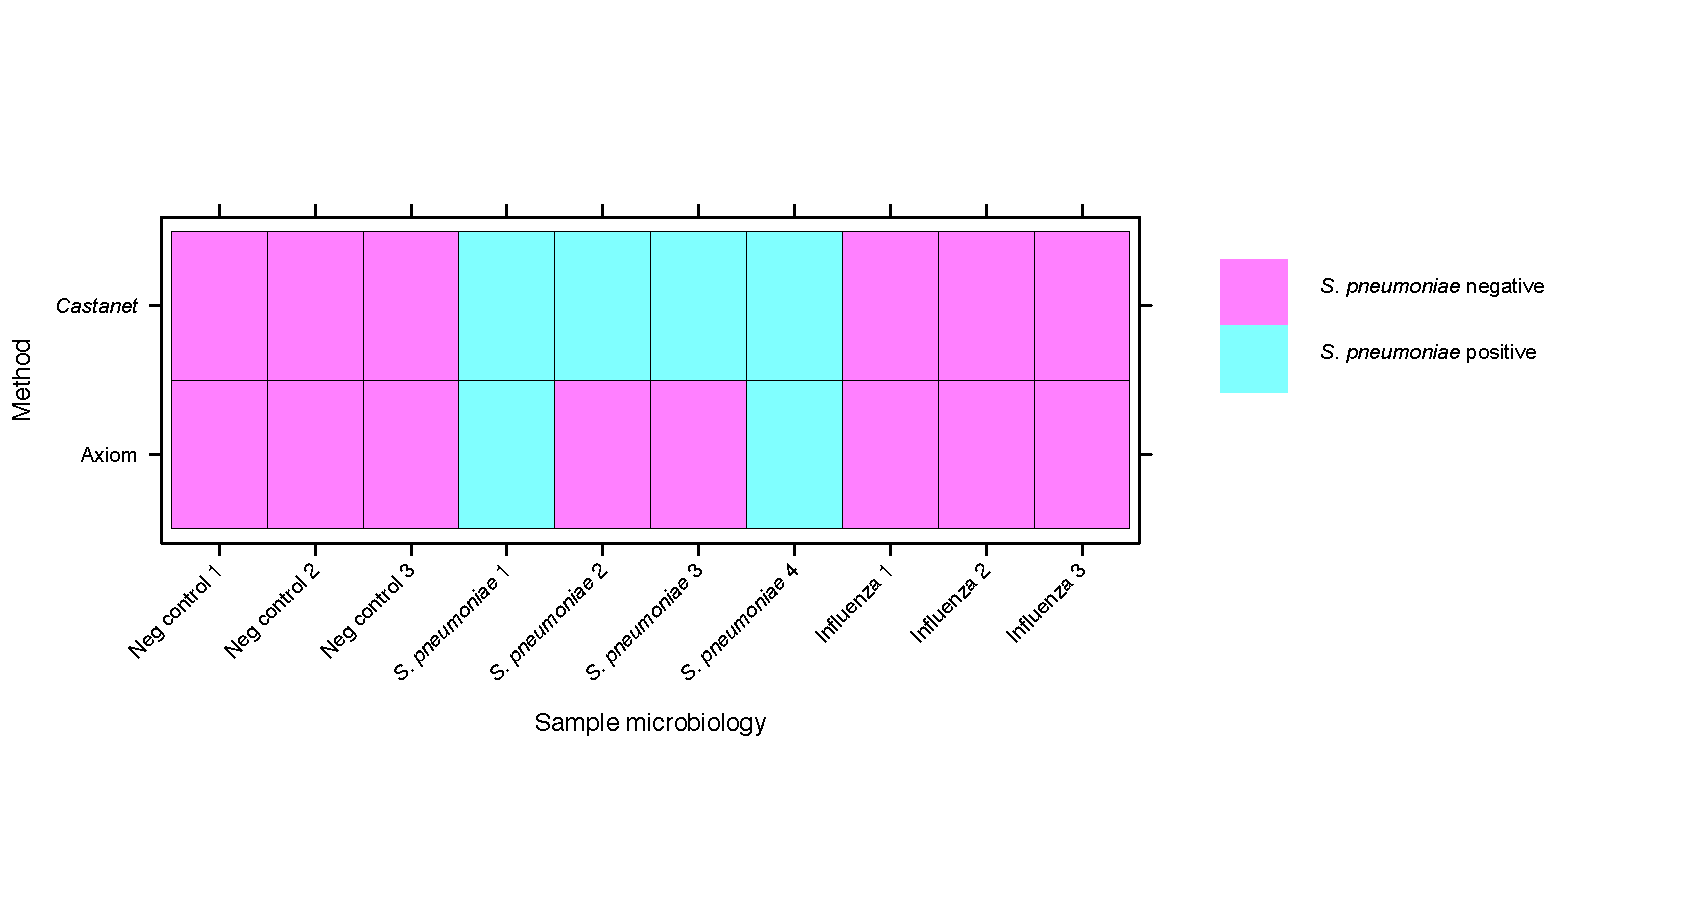
\includegraphics[scale=0.6]{./Results2/Images/Axiom.pdf}
\caption[Axiom Microbiome Array results for \textit{Streptococcus pneumoniae}]{\textbf{Axiom Microbiome Array results for\textit{Streptococcus pneumoniae} compared with \textit{Castanet}.} Clinical microbiology status and detection for \textit{S. pneumoniae} is displayed in the heatmap.}
\label{fig:axiom}
\end{figure}

In total, 10 organisms were detected across the 10 samples (Figure ~\ref{fig:axiom-summary}). The majority of organisms were of little clinical consequence, e.g. Torque teno virus and \textit{Propionibacterium acnes}. However, \textit{Escherichia coli} was detected in 9 out of 10 samples, presumably reflecting sample or reagent contamination. Quantitative data is not a feature available via the Axiom Microbial Detection Analysis Software (MiDAS). 


\begin{figure}[htbp]
\centering
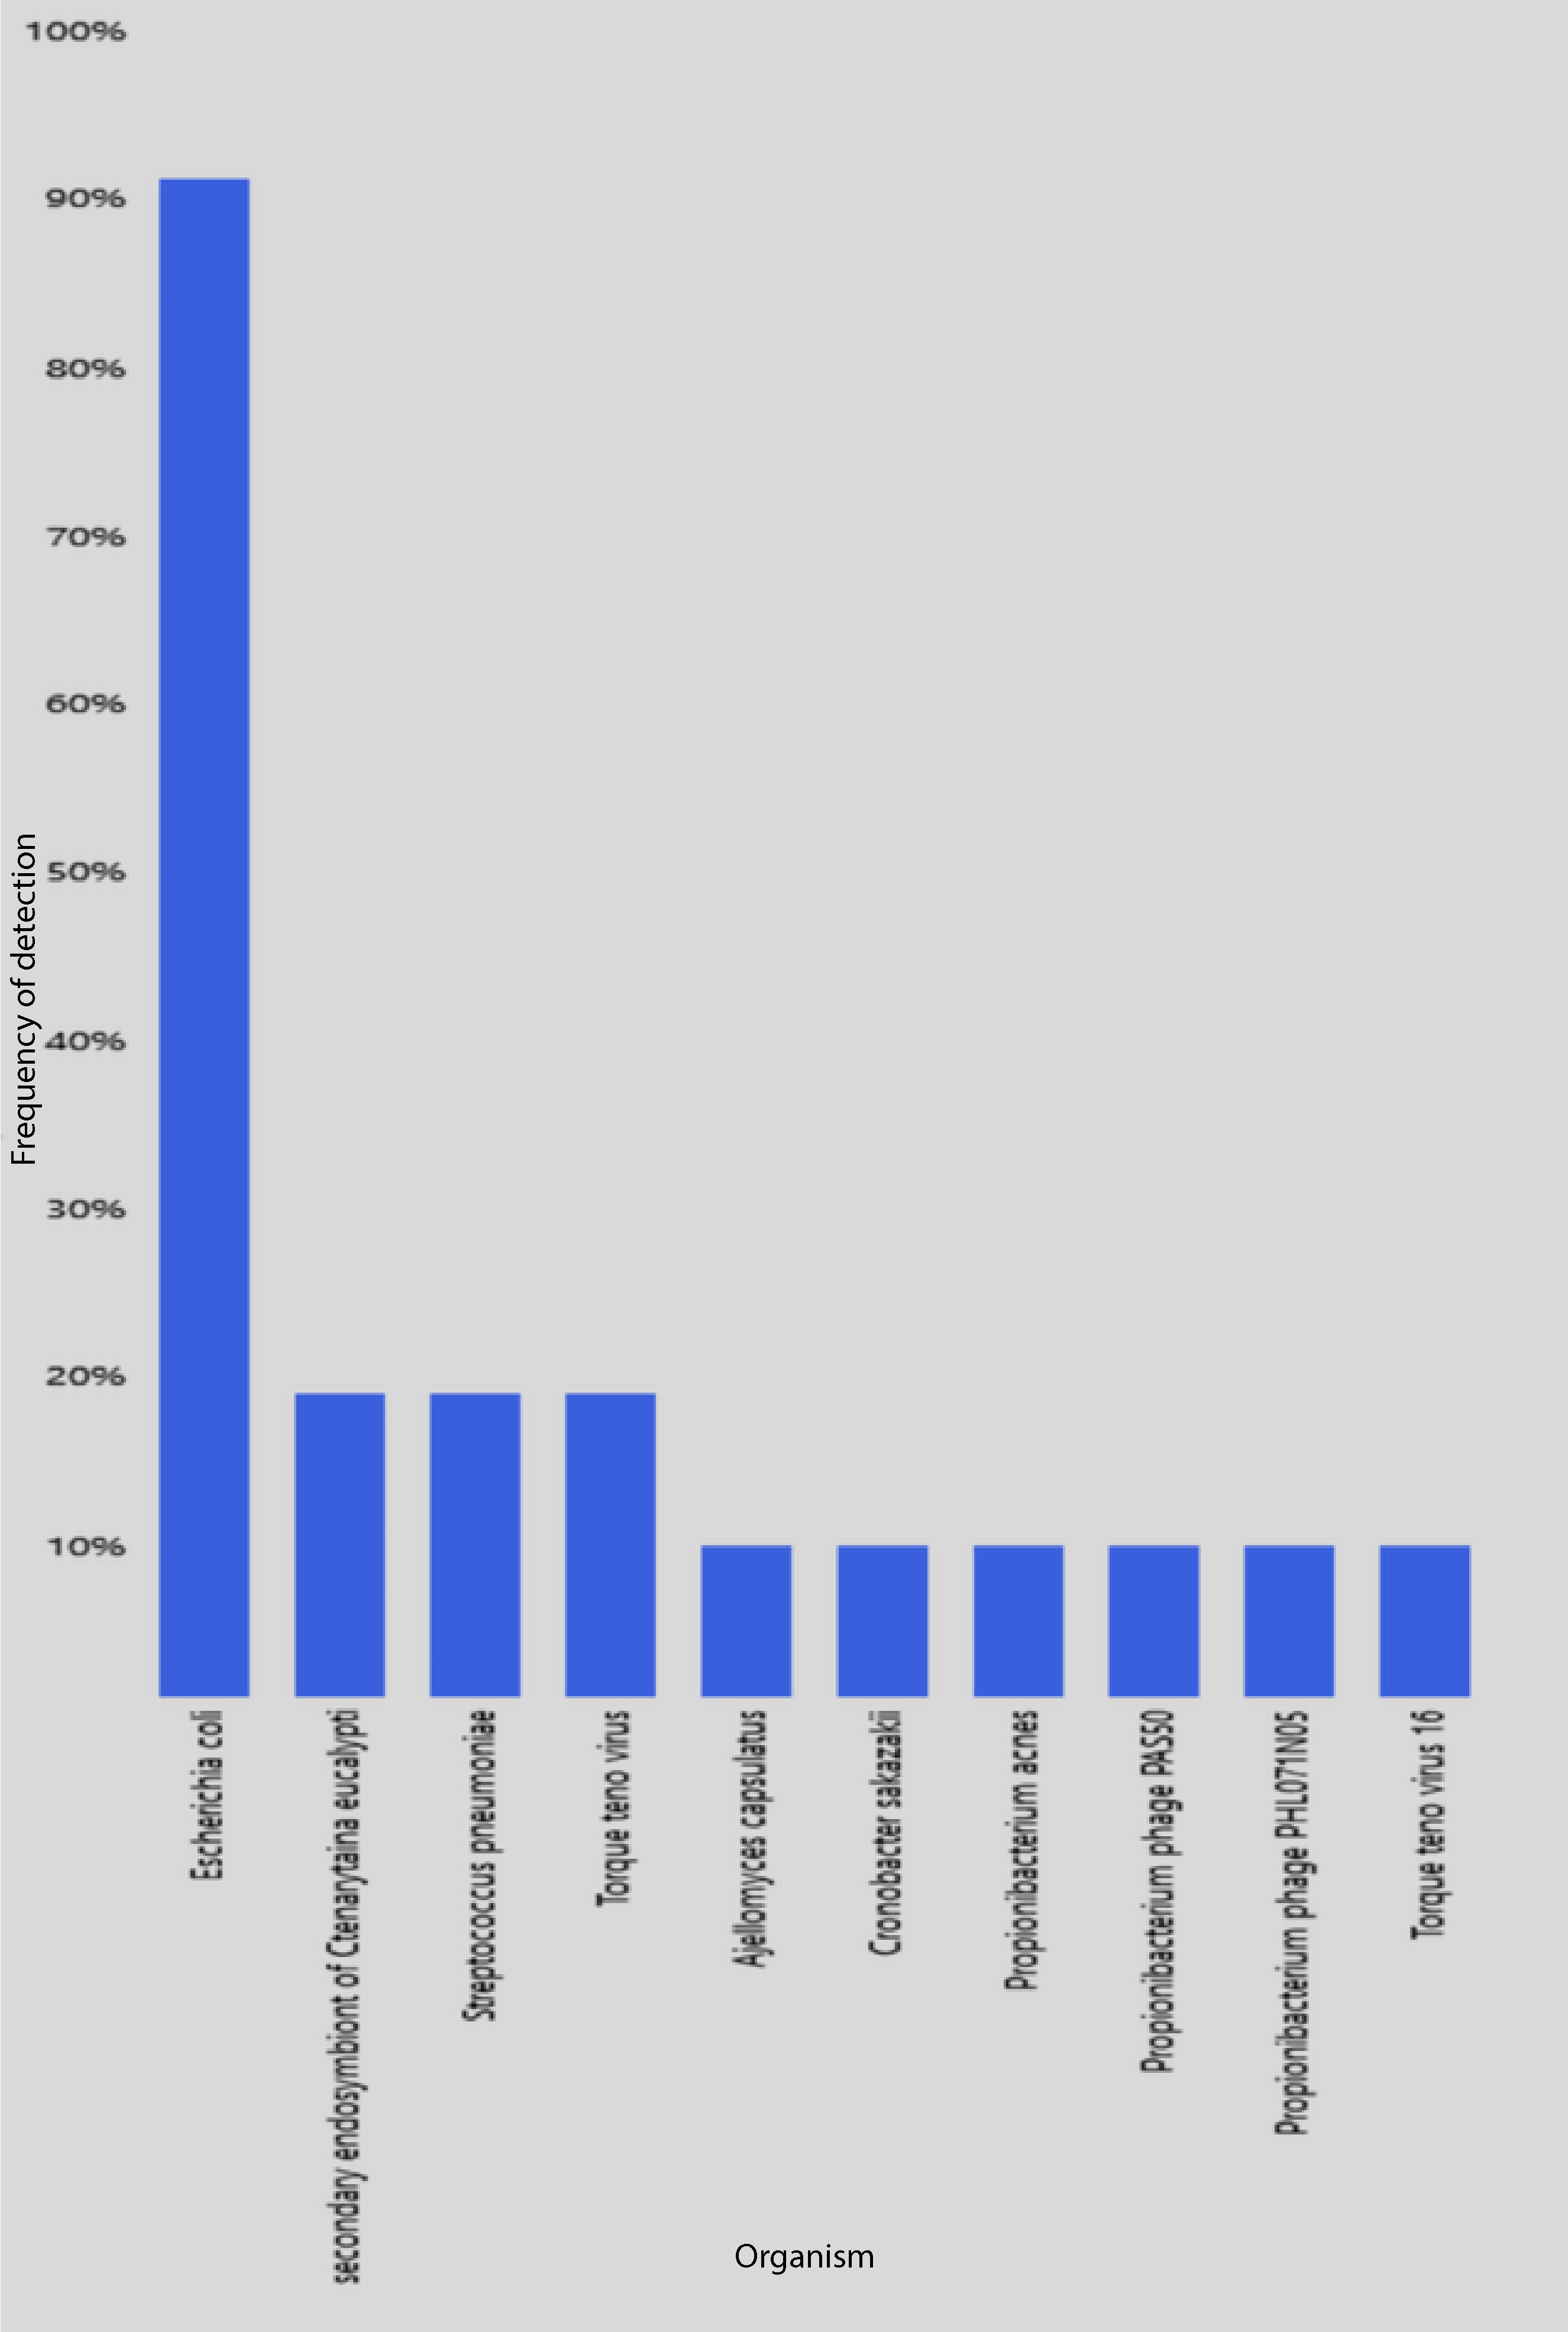
\includegraphics[scale=0.5]{./Results2/Images/MicrobeFrequencySpecies.png}
\caption[Summary of Axiom Microbiome Array results]{\textbf{Summary of Axiom Microbiome Array results.} All organisms detected in any of the 10 samples are depicted in the bar chart with the frequency of detection displayed on the y-axis.}
\label{fig:axiom-summary}
\end{figure}
\FloatBarrier
\subsection{Application to the GAinS cohort}
Of the three methods explored in this chapter (\textit{Castanet}, ddPCR, Axiom Microbiome Array), improved microbiological phenotyping for GAinS CAP sepsis patients was obtained primarily through \textit{Castanet} targeted metagenomic sequencing.

In the GAinS CAP sepsis patients undergoing metagenomic sequencing (n=573), \textit{Castanet} identified a likely causative pathogen in 176/573 (31\%) of cases. This was a 9\% improvement on the 126/573 (22\%) of cases with a microbiological diagnosis arising from clinical microbiology alone (Table ~\ref{tab:gains-summary-castanet}).

Integrating this into the GAinS CAP sepsis cohort as a whole (n=1222) (Table ~\ref{tab:clinmicro}), the application of targeted metagenomics reduced the number of individuals with no microbiology diagnosis from 729 (60\%) to 693 (57\%) (Table ~\ref{tab:gains-summary}). 
 

\FloatBarrier
\begin{table}[]
\begin{center}
\begin{tabular}{|c|c|c|c|}
\hline
\textbf{Organism}      & \textbf{\begin{tabular}[c]{@{}c@{}}Clinical \\ microbiology\end{tabular}} & \textbf{\begin{tabular}[c]{@{}c@{}}Clinical microbiology \\ + \textit{Castanet}\end{tabular}} & \textbf{\begin{tabular}[c]{@{}c@{}}Prevalence in \\ overall GAinS cohort\end{tabular}} \\ \hline
Unknown                & 447 (78\%)                                                                & 397 (69\%)                                                                           & 60\%                                                                                   \\ \hline
\textit{S. pneumoniae} & 92 (16\%)                                                                 & 108 (19\%)                                                                           & 15\%                                                                                   \\ \hline
Other bacterial        & 6 (1\%)                                                                   & 33 (6\%)                                                                             & 18\%                                                                                   \\ \hline
Influenza              & 13 (2\%)                                                                  & 14 (2\%)                                                                             & 5\%                                                                                    \\ \hline
Other viral            & 15 (3\%)                                                                  & 21 (4\%)                                                                             & 3\%                                                                                    \\ \hline
\textbf{Total}         & \textbf{573}                                                              & \textbf{573}                                                                         & 100\%                                                                                  \\ \hline
\end{tabular}
\end{center}
\smallskip
\caption[Summary of microbiology in GAinS patients undergoing \textit{Castanet} sequencing]{\textbf{Summary of microbiology in GAinS patients with sepsis due to CAP undergoing \textit{Castanet} sequencing (n=573).} The prevalence of each organism in the overall GAinS cohort (n=1222) based on clinical microbiology alone is displayed in the last column to show how the GAinS metagenomic cohort (n=573) compares in microbiology diagnosis to the overall cohort.} 
\label{tab:gains-summary-castanet}
\end{table}

\begin{table}[]
\begin{center}
\begin{tabular}{|c|c|l|}
\hline
\multirow{2}{*}{\textbf{Diagnosis}} & \multicolumn{2}{c|}{\textbf{Number of patients (\%)}}      \\ \cline{2-3} 
                                    & \textbf{With metagenomics} & \textbf{Without metagenomics} \\ \hline
Unknown                             & 693 (57)                   & 729 (60)                      \\ \hline
Bacterial                           & 426 (35)                   & 399 (33)                      \\ \hline
Viral                               & 86 (7)                     & 80 (7)                        \\ \hline
Mixed bacterial/viral               & 15 (1)                     & 12 (1)                        \\ \hline
Fungal                              & 2 (0.2)                    & 2 (0.2)                       \\ \hline
\end{tabular}
\end{center}
\smallskip
\caption[Summary of microbiology in entire cohort of GAinS patients with sepsis due to CAP] {\textbf{Summary of microbiology in entire cohort of GAinS patients with sepsis due to CAP (n=1222).} Diagnoses made on the basis of metagenomics and clinical microbiology and compared with those made on the basis of clinical microbiology only.}
\label{tab:gains-summary}
\end{table}
\FloatBarrier


\section{Discussion}
\subsection{Targeted metagenomics and droplet digital PCR}
The \textit{Castanet} workflow enabled successful sequencing of a range of bacteria and viruses (both RNA-based and DNA-based) from a subset of sepsis plasma samples. In spite of difficulties describing a 'truth dataset' of known positives and known negatives, the characteristics of pathogen-positive and pathogen-negative samples were defined using a random forest model that combines data across pathogens and diseases. In the test dataset, a specificity of 98.6\% and sensitivity of 86.7\% was observed. Similarly, high specificity (100\%) and sensitivity (83\%) was also observed when \textit{Castanet} was evaluated against a gold-standard independent method of detection (ddPCR) for \textit{S. pneumoniae}.

Despite this high sensitivity of detection, a causative organism was only identified in 11\% of plasma samples from patients who had no positive microbiology result from routine clinical microbiological testing. This was lower than the figure observed in the ChiMES cohort, where 32\% of similar samples yielded a new diagnosis with \textit{Castanet}. There are several likely explanations for this. Firstly, timing of sample collection was suboptimal for diagnostic metagenomics; the earliest time at which a plasma sample was obtained was on the first day of ICU admission after the consenting process. By this time, the diagnosis of sepsis would have been made and antimicrobial drugs administered. Secondly, the nature of the sample type would have contributed to the low diagnosis rate. In the setting of sepsis secondary to pneumonia, plasma may contain little or no pathogen material from agents such as influenza A virus where viraemia is not typically a feature of disease.

Future work to enable more comprehensive evaluation of \textit{Castanet} sequencing would include recruitment and sampling of patients at earlier time points prior to the administration of antimicrobials, with consent procedures such as emergency waiver of consent in place. In addition, sampling of other relevant specimen types for CAP sepsis (e.g. nasopharyngeal swabs for viral infections) is likely to increase the rate of pathogen detection. 

Other opportunities for future work include improving probe design to enable better resolution of pathogenic species within clusters of closely related bacteria. Currently, \textit{Castanet} is unable to differentiate between species within the \textit{Enterobacteriaceae} family or between \textit{Streptococcus pyogenes} and \textit{Streptococcus agalactiae}. This work could also focus on bacterial sequences of particular clinical interest such as factors associated with virulence and anti-microbial resistance. 

\subsection{Axiom Microbiome Array}
Compared with \textit{Castanet}, the Axiom Microbiome Array had low sensitivity (50\%) for \textit{S. pneumoniae} detection. This may have been because the manufacturers recommend a quantity of 50-100ng DNA per sample which was unachievable in this experiment, given the low DNA quantities (2-20ng) usually obtained following  nucleic acid extraction of the typical 500$\mu$l aliquot of plasma received from the recruiting centres. Other disadvantages include the absence of quantitative data, meaning it was difficult to determine whether the presence of \textit{E. Coli} was as a contaminant or pathogenic. Also, separate workflows (and thus increased sample volumes) are required for RNA and DNA pathogens. These disadvantages outweighed the main benefit of the Axiom Microbiome Array which included the straightforward sample processing, data generation and analysis steps.

For analysis of sample types like plasma from sepsis patients where sensitivity is a major challenge and specimen volumes are limited, the Axiom Microbiome Array is not a suitable method for diagnostics.

\section{Conclusions}
In the GAinS cohort of sepsis CAP patients, the majority of individuals (60\%) lack a microbiological diagnosis despite extensive laboratory testing. In this chapter, I have shown that although there are limitations, targeted metagenomics enables new diagnoses to be made in this challenging cohort using the \textit{Castanet} workflow. This has important clinical and scientific implications, enabling more accurate prescribing of antimicrobial therapy and better understanding of disease heterogeneity. 
